%%%%%%%%%%%%%%%%%%%%%%%%%%%%%%%%%%%%%%%%%%%%%%%%%%%%%%%%%%%%%%%%%%%%%%%%%%%

\documentclass{standalone}

\usepackage{mathptmx}
\usepackage{tikz}
\usetikzlibrary{external}
\tikzexternalize{number-tree}

%% We default to Times.
\renewcommand{\rmdefault}{ptm}
\renewcommand{\ttdefault}{pcr}
%% Enable Times/Palatino main text font.
\normalfont\selectfont

%% A tree that represents the hierarchy of real numbers.

\begin{document}

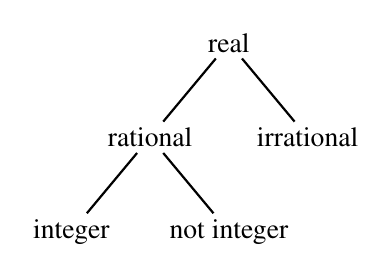
\begin{tikzpicture}[%%
  lineStyle/.style={-,thick},%%
  nodeStyle/.style={inner sep=2pt}%%
]
%%
%%
\pgfmathsetmacro{\dy}{1.2}
%%
\coordinate (Integer) at (0,0);
\coordinate (Irrational) at (3,\dy);
\coordinate (NotInteger) at (2,0);
\coordinate (Rational) at (1,\dy);
\coordinate (Real) at (2,2*\dy);
%%
%%
%% Draw the number tree.
%% Nodes of the number tree.
\node (NotQQ) at (Irrational) [nodeStyle] {irrational};
\node (NotZZ) at (NotInteger) [nodeStyle] {not integer};
\node (QQ) at (Rational) [nodeStyle] {rational};
\node (RR) at (Real) [nodeStyle] {real};
\node (ZZ) at (Integer) [nodeStyle] {integer};
%% Lines between the nodes.
\draw[lineStyle] (QQ) edge node {} (ZZ);
\draw[lineStyle] (QQ) edge node {} (NotZZ);
\draw[lineStyle] (RR) edge node {} (QQ);
\draw[lineStyle] (RR) edge node {} (NotQQ);
\end{tikzpicture}

\end{document}
